\section{GUI}
\label{appendix:GUI}
\subsection{GUI Code}
\label{appendix:GUICode}
\counterwithin{figure}{section}
\lstset{basicstyle=\tiny}
\begin{lstlisting}[language=Python,caption={GUI.py},label={lst:GUI.py}]
#Written by Brendon Camm, last updated April 9th, 2017

import sys
from PyQt5 import QtCore, QtGui, uic, QtWidgets
import numpy as np
import time
import struct
import socket
from PS4_Controller import PS4Controller as PS4
import pyqtgraph as pg
import pyqtgraph.exporters

qtCreatorFile = "GUI.ui" # Enter QtDesigner file here.
Ui_MainWindow, QtBaseClass = uic.loadUiType(qtCreatorFile)



class GUI(QtWidgets.QMainWindow, Ui_MainWindow, QtWidgets.QMenu):   
def __init__(self):

super(GUI,self).__init__()
#Qt initialization
QtWidgets.QMainWindow.__init__(self)
Ui_MainWindow.__init__(self)
self.page = QtWidgets.QStackedWidget()
self.setCentralWidget(self.page)
self.setupUi(self)
self.setWindowTitle("Drone")
self.setWindowIcon(QtGui.QIcon('smu.png'))

#Networking
self.getHost = socket.gethostname()
self.staticPort = '1247'

#Main Page buttons
self.start.clicked.connect(self.connection)
self.end.clicked.connect(self.stop)

#Listing widget, allows for the user to select a certain page
self.list.insertItem(0, 'Home')
self.list.insertItem(1, 'Controller')
self.list.currentRowChanged.connect(self.display) #Changes widget index to appropriate page

#Controller Page
self.axisVal.setText('1 2 3 4')
self.hostVal.setText(self.getHost)
self.portVal.setText(self.staticPort)
self.axisMenu.clicked.connect(self.axisSettings) #When "Update Axis" is clicked call definition axisSettings
self.hostMenu.clicked.connect(self.hostSettings) #When "Update host" is clicked call definition hostSettings
self.portMenu.clicked.connect(self.portSettings) #When "Update Port" is clicked call definition portSettings
self.updateConnect.clicked.connect(self.updateConnection) #When "Update Connection" is clicked call definition updateConnection
self.connectPS4.clicked.connect(self.connectController) #When "Manual Control" is clicked call definition connectController

#Live plotting Initializations
self.initplt()
self.plotcurve = pg.PlotDataItem()
self.plotwidget.addItem(self.plotcurve)
self.t = 0
self.update1()
self.timer = pg.QtCore.QTimer()
self.timer.timeout.connect(self.move)# Connects a timer to the "move" definition that allows for live plotting
self.timer.start(1000) # Poll for updates of new data ever 1000miliseconds (1 second)

def stop(self):
sys.exit(app.exec_())

def connection(self):
s = socket.socket()
host = self.getHost
port = int(self.staticPort)
status = s.connect_ex((host,port)) #Returns 0 if connect is successful, returns errno if not
if status: # Status = errno
self.thisworks.setText("Connection Unsuccessful")
self.connectionStat.setText("Communications have not been established")
else: # Status = 0
print(status)
self.thisworks.setText("Connection Successful")
self.connectionStat.setText("Communications are active")

def axisSettings(self):
cont = PS4()
#Input boxes when "Update Axis" is clicked
text, ok = QtWidgets.QInputDialog.getText(self, 'Axis Value[0]', 'No Spaces')
text1, ok = QtWidgets.QInputDialog.getText(self, 'Axis Value[1]', 'No Spaces')
text2, ok = QtWidgets.QInputDialog.getText(self, 'Axis Value[2]', 'No Spaces')
text3, ok = QtWidgets.QInputDialog.getText(self, 'Axis Value[3]', 'No Spaces')
axis = [int(text), int(text1), int(text2), int(text3)] # Make an array of the values from the input dialogs
self.axisVal.setText(str(axis)) 
cont.axis_order = axis # Set the axis order for the controller equal to the new settings

def display(self,i):
self.home.setCurrentIndex(i)

def hostSettings(self):
#Input box when "Update Host" is clicked
text, ok = QtWidgets.QInputDialog.getText(self,'Host', 'Host name or IP address')
newHost = str(text)
if newHost == '':
self.hostVal.setText(self.getHost)
else:
self.hostVal.setText(newHost)
return newHost

def portSettings(self):
#Input box when "Update Port" is clicked
text, ok = QtWidgets.QInputDialog.getText(self,'Port','Port number')
if ok:
print('success')
newPort = str(text)
if newPort == '':
self.portVal.setText(self.staticPort)
else:
self.portVal.setText(newPort)     
return int(newPort)

def connectController(self):
new = PS4()
cont.axis_order = self.axisSettings()
print(str(cont.axis_order))
new.listen() #Accept data from the manual controller, calls the listen definition from PS4Controller.py

def updateConnection(self):
host1 = self.hostSettings()
port1 = self.portSettings()
s = socket.socket()
status = s.connect_ex((host1,port1)) #Returns 0 if connect is successful, returns errno if not

if status: #status = errno
self.connectionStat.setText("Update and Connection Unsuccessful")
self.thisworks.setText("Update and Connection Unsuccessful")
else: #status = 0
self.connectionStat.setText("Update and Connection Successful")
self.thisworks.setText("Update and Connection Successful")

def liveData(self):
graph_data = open('test.txt', 'r').read() # Open the text file to read in data
lines = graph_data.split('\n') # Read in data from different lines
xs = [] #Empty list
ys = [] #Empty List
for line in lines:
if len(line)>1:
x, y = line.split(' ,') #Read in data in the form of (x ,y)
xs.append(int(x))
ys.append(int(y))
return xs,ys

def initplt(self):
self.plotwidget = pg.PlotWidget() #Initate the plotting widget field
self.mplvl.addWidget(self.plotwidget) #Set the plotting widget field to populate the QVBoxLayout widget field
self.plotwidget.setLabel('left', 'Altitude [m]') # Y-Axis name
self.plotwidget.setLabel('bottom','Time[s]') #X-Axis name
self.show()

def update1(self):
#read in the data from the liveData definition in the form of two separate lists. 
#list1 = x-values, list2 = y-values
list1,list2 = self.liveData()
self.plotcurve.setData(list1,list2) # Plot the data

def move(self):
self.t+=1 #Move the data 1 spot to the right
self.update1() # Call update1 definition to get the new data


if __name__ == '__main__':
app = QtWidgets.QApplication(sys.argv)
main = GUI()
main.show()
QtWidgets.QApplication.processEvents()
sys.exit(app.exec_())
\end{lstlisting}
\begin{figure}[H]
	\label{fig:OGUIHomePage}
	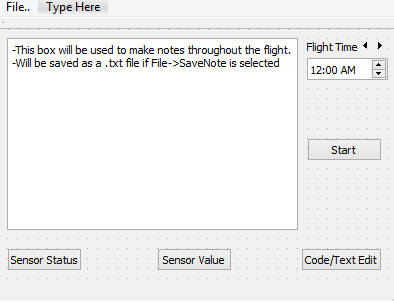
\includegraphics[width=\linewidth]{OLDGUI1.png}
	\caption{Original GUI Prototype Home Page}
\end{figure}
\begin{figure}[H]
	\label{fig:OGUIPage2}
	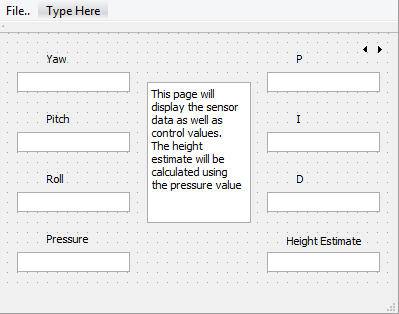
\includegraphics[width=\linewidth]{OLDGUI2.png}
	\caption{Original GUI Prototype 2nd Page}
\end{figure}
